\chapter{Invasive attacks}
As already stated in chapter \ref{ch:hw-attacks-taxonomy}, invasive attacks are a kind of hardware
attacks that require actions against the attacked hardware to allow physical intrusions to access
some internal components easily.\\
They usually require a relatively high investment in terms of lab equipment and moderate effort.
Some examples of this kind of attacks are micro probing, reverse engineering and data remanence
attacks.
\begin{section}{Micro probing}
  \begin{boxH}
    \textbf{Micro probing} is a type of physical attack that directly probes the signal wires inside
    the chip in order to extract sensitive information.
  \end{boxH}
  One can try to do so by exposing the die by removing the plastic package via chemical or
  mechanical means, and then measuring electrical quantities directly on it.
  \begin{figure}[H]
    \centering
    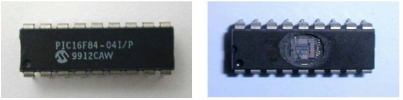
\includegraphics[width=0.5\textwidth]{img/hardware/depackaged chip.png}
    \caption{A comparison between a packaged and a depackaged chip}
    \label{fig:depackaged-chip}
  \end{figure}
  Microprobing-based attacks can, in turn, be:
  \begin{itemize}
    \item Passive: e.g., using microprobes to monitor a smartcard’s bus while a program is executing
    \item Active: in this case, signals may also be injected, the classic example being the use of a
      grounded microprobe needle on the clock line to the instruction latch to disable jump
      instructions.
  \end{itemize}

\end{section}
\begin{section}{Reverse engineering}
  \begin{boxH}
    \textbf{Reverse engineering} is the process involving the thorough examination of an object to
    achieve a full understanding of its construction and/or functionality.
  \end{boxH}
\end{section}

\begin{section}{Data Remanence}
  \begin{boxH}
    \textbf{Data remanence} is the residual representation of data that remains even after attempts
    have been made to remove or erase the data.
  \end{boxH}
  This residue may result from:
  \begin{itemize}
    \item data being left intact by a nominal file deletion operation
    \item by reformatting of storage media that does not remove data previously written to the media
    \item through physical properties of the storage media that allow previously written data to be
      recovered
  \end{itemize}
  An attacker with physical access to a computing system may just disconnect the memory chips and
  then retrieve their content at disconnection time by analyzing them off-line.
  \begin{subsection}{Cold boot attack}
    \begin{boxH}
      A \textbf{cold boot attack} is a process for obtaining unauthorized access to a computer's
      encryption keys when the computer is left physically unattended.
    \end{boxH}
    Contrary to popular assumption, DRAMs used in most modern computers retain their contents for
    several seconds after power is lost, even at room temperature and if removed from a motherboard.
    Although DRAMs become less reliable when refreshed, they are not immediately erased, and their
    contents persist sufficiently for malicious (or forensic) acquisition of usable full-system
    memory images.

    \begin{figure}[H]
      \centering
      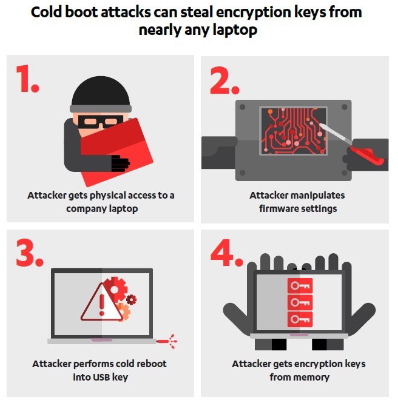
\includegraphics[width=0.5\textwidth]{img/hardware/cold boot attack.png}
      \caption{Cold boot attack}
      \label{fig:cold-boot-attack}
    \end{figure}
  \end{subsection}

\end{section}
